\chapter{Background}\label{ch:background}
%************************************************ 

\section{Neural networks as classifiers}

	One of the most popular use cases of \acs{ANN}s is supervised learning; what distinguishes it from unsupervised learning is the existence of labeled examples that guide the learning stage, against the need to infer all information. Supervised learning can be further divided into classification and regression: the former aims to split a set of data into two or more groups, while the latter is more of a function approximation. Since our job will consist in recognizing several types of \acs{EEG} patterns, the discussion will focus on the particular details of classification from here on.

	A neural network, in its most basic form, is made of simple processing units (called \textit{neurons}) distributed among three kinds of layers:

	\begin{itemize}

		\item
		Input layer: with as many neurons as characteristics describing a single sample. Each unit receives the value of its corresponding characteristic as is. Depending on the problem (and not just for this sort of model), it may be useful to preprocess the data so as not to bias the model.

		\item
		Output layer: the number of possible outputs dictates its number of neurons. Only one of them can be active at a time, indicating the answer of the neural network to the classification question.

		\item
		Hidden layers: these are inserted between the previous two. Their quantity ranges from one to hundreds in the most extreme applications, and their interactions yield the predictive ability of the model.

	\end{itemize}

	A typical vanilla feed-forward neural network contains directed connections between its different layers, but not between components of the same layer. Also, the term \textit{feed-forward} implies that there are no cycles in the graph of the network, and so the information moves from the input to the output through the hidden layers. The way in which this information flows is defined by the \textit{activation function} (the response of a neuron from an input number) as well as the \textit{weights} of the connections between neurons: although it is frequent to have fully-connected layers, it does not mean that one unit passes the same value to all the other units it points to, or even that they are not null; determining that is precisely the task of the learning algorithm.

\newpage

	To get a better picture of the concept, the following figure illustrates a generic model with one hidden layer:

	\vspace{0.2cm}

	\begin{figure}[bth]

        \myfloatalign
        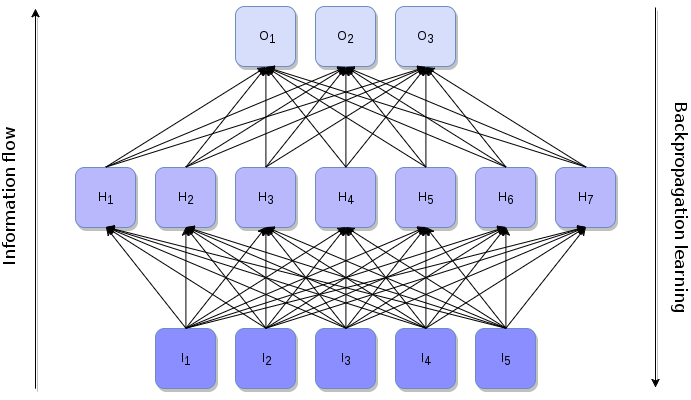
\includegraphics[width=0.9\textwidth]{gfx/NeuralNetwork.png}
        \caption{A neural network with one hidden layer.}

    \end{figure}

    We can see that the hidden layer has its neurons labeled $H_i$. The input layer is represented by the $I_i$ units and the output layer corresponds to the different $O_i$. 

    This image introduces another new concept: \textit{backpropagation}. Whereas the information is transformed by means of the weights and transmitted forward, the adjustment of those weights also needs of a propagation in the opposite direction. To sum it up, backpropagation has two main steps:

    \begin{enumerate}

    	\item
    	Propagation. Generate predictions for the training examples, then calculate the error at the output layer; a common error measure is the squared difference between the actual value and the expected value. Afterwards, recursively propagate the error calculations to the successive hidden layers taking into acount the already computed error values, until the input layer is reached.

    	\item
    	Weight update. Multiply the value of the activation function of each neuron and its error obtained in the first step. This is called the \textit{gradient} in \textit{Gradient Descent}. Finally, subtract a fraction of this gradient from the weight; that fraction (\textit{learning rate}) has a significant effect on the process, for a value too high can cause the algorithm to jump over a local minimum without reaching it, and a value too low can overextend the training time.

    \end{enumerate}

    The above procedure is repeated until the model's performance is adequate. If we wish to speed it up with a reasonable tradeoff in quality, we can use not the whole training set for each iteration but smaller subsets called \textit{batches} (\textit{Stochastic Gradient Descent}). This allows us to maintain enough generalization while at the same time reducing the cost of gradient computation \cite{lecun-dl}.

    In general, as the complexity of a model grows, so does the difficulty of its training. Neural networks are, in theory, capable of approximating every possible function, and this comes at a price: some of the following common issues in machine learning \cite{nn-atc} have increased consequences.

    \begin{itemize}

    	\item
    	Limited data: without delving too much into the underlying theory, the more powerful a model is, the more training samples are needed in a substantial proportion. Coupled with it, the smaller the training set, the smaller the chance that it will represent the whole population.

    	\item
    	Imbalanced data: when there are far more examples of one or more classes than of the rest, we speak of imbalance. Apart from not representing the population, this phenomenon can even bias a classifier in a way that it only outputs one class, as it seems the best way to minimize the error.

    	\item
    	Incomplete data: this is the case when the available samples have missing values. In this situation there are two options: either we discard incomplete fields from across all samples or we try to infer them.

    	\item
    	High dimensionality: linking with the first bullet point, powerful models can suffer of \textit{overfitting} with limited and/or high-dimensional samples. The latter can cause the model to just learn the available data ``by heart'' and fail to generalize to new examples.

    \end{itemize}

    Another problem is the \textit{vanishing gradient}, which occurs only in the training stage of neural networks. Because of the chain rule used to propagate the error through the layers, if the activation function provides many values close to zero, the gradient will approach that value too. In worst-case scenarios, it results in a practical standstill of the training. Plausible solutions to this matter, which has been a major deterrent against deep architectures for a long time, include the use of alternative activation functions (such as \textit{ReLU} and its variants, very popular in recent years \cite{delv-deep-relu,deep-res-relu}).